% (c)~2014 Claudio Carboncini - claudio.carboncini@gmail.com
% (c)~2014 Dimitrios Vrettos - d.vrettos@gmail.com
% (c) 2015 Daniele Zambelli daniele.zambelli@gmail.com

% \section{Esercizi}
% 
% \subsection{Esercizi dei singoli paragrafi}
% 
% \subsubsection*{\numnameref{sec:01_}}
% 
% \begin{esercizio}
% \label{ese:D.19}
% testo esercizio
% \end{esercizio}
% 
% \begin{esercizio}\label{ese:03.1}
% Consegna:
%  \begin{enumeratea}
%   \item  
%  \end{enumeratea}
% \end{esercizio}
% 
% \subsection{Esercizi riepilogativi}
% 
% \begin{esercizio}
% \label{ese:D.19}
% testo esercizio
% \end{esercizio}
% 
% \begin{esercizio}\label{ese:03.1}
% Consegna:
%  \begin{enumeratea}
%   \item  
%  \end{enumeratea}
% \end{esercizio}

\section{Esercizi}
\subsection{Esercizi dei singoli paragrafi}
% \subsection*{4.1 - Risoluzione delle disequazioni di secondo grado}
\numnameref{sec:diseq_secondo_grado}

\begin{esercizio}
 \label{ese:4.7}
Rappresentare nel riferimento cartesiano ortogonale le seguenti parabole.
\begin{multicols}{2}
 \begin{enumeratea}
 \item~$ y=-3x^2+x $
 \item~$ y=\frac 1 2x-2x+\frac 3 2 $
 \item~$ y=x^2+x-1 $
 \item~$ y=x^2-x+1 $
 \end{enumeratea}
 \end{multicols}
\end{esercizio}

\begin{esercizio}
 \label{ese:4.8}
Rappresentare nel riferimento cartesiano ortogonale le seguenti parabole.
\begin{multicols}{2}
 \begin{enumeratea}
 \item~$ y=-3x^2+3 $
 \item~$ y=x^2+4x+3 $
 \item~$ y=x^2+\frac 3 5 $
 \item~$ y=-\frac 2 5x^2+4x-\frac 1 5 $
 \item~$ y=-\frac 1 2 x^2-4x-1 $
 \end{enumeratea}
 \end{multicols}
\end{esercizio}

\begin{esercizio}
 \label{ese:4.9}
Per ciascun grafico di parabola $y=ax^2+bx+c$ indica il segno del primo 
coefficiente e del discriminante, la natura dei suoi zeri (reali distinti, 
reali coincidenti, non reali), il segno della funzione.
\begin{center}
 % (c) 2012 Dimitrios Vrettos - d.vrettos@gmail.com
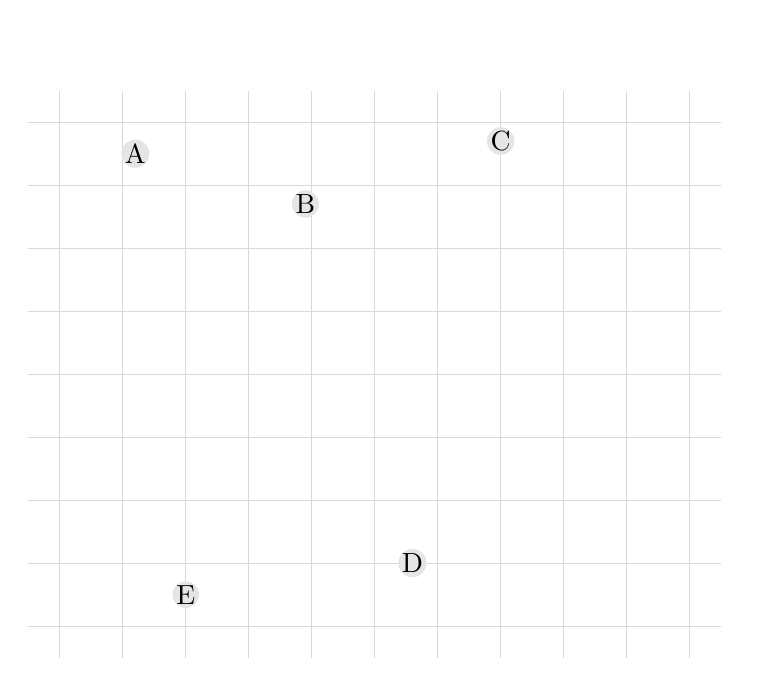
\begin{tikzpicture}[x=8mm, y=8mm]
\draw[step=0.8cm,color=gray!30] (-5.5,-4.5) grid (5.5,4.5);
  \tkzInit[xmin=-5,xmax=5,ymin=-4.5,ymax=4.5]
  \clip (-5.5,-4.5) rectangle (6,5.5);
  \begin{scope}[font=\small]
    \tkzAxeY[orig = false, label options={left = 1pt}]
    \tkzAxeX[orig = true, label options={below = 1pt}]
  \end{scope}
  \tkzFct[domain=-1.5:1.5,thick,color=darkgray]{2*x*x-1}
  \node [inner sep=0pt, circle, fill=gray!20] (a) at (-1.1, 2.7) {B};
  \tkzFct[domain=0:3,thick,color=blue]{-2*x*x+6*x-4};
  \node [inner sep=0pt, circle, fill=gray!20] (a) at (.6, -3) {D};
  \tkzFct[domain=-3.3:-.7,thick,color=RedOrange]{-2*x*x-8*x-8.5};
  \node [inner sep=0pt, circle, fill=gray!20] (a) at (-3, -3.5) {E};
  \tkzFct[domain=1.5:4.5,thick,color=purple]{2*x*x-12*x+18};
  \node [inner sep=0pt, circle, fill=gray!20] (a) at (2, 3.7) {C};
  \tkzFct[domain=-4.5:-1.5,thick,color=olive]{2*x*x+12*x+19};
  \node [inner sep=0pt, circle, fill=gray!20] (a) at (-3.8, 3.5) {A};

\end{tikzpicture}

\end{center}
\end{esercizio}

\begin{esercizio}[\Ast]
 \label{ese:4.1}
Risolvi le seguenti disequazioni di secondo grado.
\begin{multicols}{2}
 \begin{enumeratea}
 \item~$x^2-6x\le 0$ \hfill $\left[0\le x\le 6\right]$
 \item~$5x^2>0$ \hfill $\left[x\neq 0\right]$
 \item~$x^2+x>0$ \hfill $\left[x<-1\vee x>0\right]$
 \item~$x^2\le 0$ \hfill $\left[x=0\right]$
 \item~$3x^2\le -1$ \hfill $\left[\emptyset \right]$
 \item~$x^2-9>0$ \hfill $\left[x_1<-3\vee x>3\right]$
 \item~$2x^2-3x+1>0$ \hfill $\left[x<\frac 1 2\vee x>1\right]$
 \item~$-x^2+3x\ge 0$ \hfill $\left[0\le x\le 3\right]$
 \item~$3x^2+x-2>0$ \hfill $\left[x_1<-1\vee x>\frac 2 3\right]$
 \item~$x^2-4>0$ \hfill $\left[x_1<-2\vee x>2\right]$
 \item~$\frac 4 3x^2-\frac 1 3x-1<0$ \hfill $\left[-\frac 3 4<x<1\right]$
 \item~$x^2-8\le 0$ \hfill $\left[-2\sqrt 2\le x\le 2\sqrt 2\right]$
%  \item~$x^2-5x+3\ge 0                          $ ZERI IRRAZIONALI
%  \hfill $\left[x\le \frac{5-\sqrt{13}} 2\vee x\ge \frac{5+\sqrt{13}} 2\right]$
 \item~$x^2-4x+9>0$ \hfill $\left[\insR\right]$
 \item~$x^2-6x+8\le 0$ \hfill $\left[2\le x\le 4\right]$
 \item~$x^2+3x-4\ge 0$ \hfill $\left[x\le -4\vee x\ge 1\right]$
 \item~$x^2-4x-9\le 0$ \hfill $\left[2-\sqrt{13}\le x\le 2+\sqrt{13}\right]$
 \item~$x^2-9x+18<0$ \hfill $\left[3<x<6\right]$
 \end{enumeratea}
 \end{multicols}
\end{esercizio}

\begin{esercizio}[\Ast]
 \label{ese:4.4}
Risolvi le seguenti disequazioni di secondo grado.
\begin{multicols}{2}
 \begin{enumeratea}
 \item~$x^2-8x+15\ge 0$ \hfill $\left[x\le 3\vee x\ge 5\right]$
 \item~$-2x^2\ge 0$ \hfill $\left[x=0\right]$
 \item~$3x^2-\frac 2 3x-1\le 0$ 
  \hfill $\left[\frac{1-2\sqrt 7} 9\le x\le \frac{1+2\sqrt 7} 9\right]$
 \item~$x^2+5>0$ \hfill $\left[\insR\right]$
%  \item~$x^2+6x-2>0$ \hfill $\left[x<-3-\sqrt{11}\vee x>-3+\sqrt{11}\right]$
 \item~$2x^2+5x+4\le 0$ \hfill $\left[\emptyset\right]$
 \item~$x^2-3x-\frac 5 2<0$ 
  \hfill $\left[\frac{3-\sqrt{19}} 2<x<\frac{3+\sqrt{19}} 2\right]$
 \item~$x^2+1>0$ \hfill $\left[\insR\right]$
 \item~$-x^2+5\le 0$ \hfill $\left[x\le -\sqrt 5\vee x\ge \sqrt 5\right]$
 \item~$x^2+x\ge 0$ \hfill $\left[x\le -1\vee x\ge 0\right]$
 \item~$(x+1)^2\ge 0$ \hfill $\left[\insR\right]$
 \item~$x^2>1$ \hfill $\left[x<-1\vee x>1\right]$
 \item~$2x^2-6<0$ \hfill $\left[-\sqrt 3<x<\sqrt 3\right]$
 \item~$-x^2-1\le 0$ \hfill $\left[\insR\right]$
 \item~$9-4x^2\le 0$ \hfill $\left[\right]$
 \item~$3x-2x^2>0$ \hfill $\left[\right]$
 \item~ $x^2\ge 0$ \hfill $\left[\right]$
 \item~$2x^2+4>0$ \hfill $\left[\right]$
 \item~$x^2-x-2>0$ \hfill $\left[\right]$
 \item~$x^2+11x+30\le 0$ \hfill $\left[\right]$
 \end{enumeratea}
 \end{multicols}
\end{esercizio}

% \subsection*{4.2 - Risoluzione grafica di una disequazione di secondo grado}
% 
% \begin{esercizio}
%  \label{ese:4.10}
% Risolvere graficamente le seguenti disequazioni di secondo grado.
% \begin{multicols}{2}
%  \begin{enumeratea}
%  \item~$ 2x^2+3x-1<0 $
%  \item~$ x^2-5x+6\le 0 $
%  \item~$ x^2-3x-4>0 $
%  \item~$ x^2-6x+5\ge 0 $
%  \end{enumeratea}
%  \end{multicols}
% \end{esercizio}
% 
% \begin{esercizio}
%  \label{ese:4.11}
% Risolvere graficamente le seguenti disequazioni di secondo grado.
% \begin{multicols}{2}
%  \begin{enumeratea}
%  \item~$ 6x^2+x-2>0 $
%  \item~$ 15x^2+x-6\le 0 $
%  \item~$ -x^2+1\ge 0 $
%  \item~$ x^2-\frac 1 4>0 $
%  \end{enumeratea}
%  \end{multicols}
% \end{esercizio}
% 
% \begin{esercizio}
%  \label{ese:4.12}
% Risolvere graficamente le seguenti disequazioni di secondo grado.
% \begin{multicols}{2}
%  \begin{enumeratea}
%  \item~$ x^2-\frac 1 4x\le 0 $
%  \item~$ x^2+2x\le 0 $
%  \item~$ x^2+2x+1\le 0 $
%  \item~$ x^2+x+1<0 $
%  \end{enumeratea}
%  \end{multicols}
% \end{esercizio}
% 
% \begin{esercizio}[\Ast]
%  \label{ese:4.13}
% Risolvi le disequazioni di secondo grado con il metodo algebrico o con quello 
% grafico.
% \begin{multicols}{3}
%  \begin{enumeratea}
%  \end{enumeratea}
%  \end{multicols}
% \end{esercizio}
% 
% \begin{esercizio}[\Ast]
%  \label{ese:4.14}
% Risolvi le disequazioni di secondo grado con il metodo algebrico o con quello 
% grafico.
% \begin{multicols}{3}
%  \begin{enumeratea}
%  \item~$-x^2+4x+3>0$
%  \item~$x^2+4x+4<0$
%  \item~$x^2-x+1<0$
%  \item~$x^2-\frac 1 9\ge 0$
%  \item~$9x^2+3x-2\le 0$
%  \item~$2x^2+5<0$
%  \end{enumeratea}
%  \end{multicols}
% \end{esercizio}
% 
% \begin{esercizio}[\Ast]
%  \label{ese:4.15}
% Risolvi le disequazioni di secondo grado con il metodo algebrico o con quello 
% grafico.
% \begin{multicols}{2}
%  \begin{enumeratea}
%  \item~$4x-x^2\ge 0$
%  \item~$9x^2+10x+1\le 0$
%  \item~$0,01x^2-1>0$
%  \item~$1,\bar 6x^2-2x\le 0$
%  \end{enumeratea}
%  \end{multicols}
% \end{esercizio}
% 
% \begin{esercizio}[\Ast]
%  \label{ese:4.16}
% Risolvi le disequazioni di secondo grado con il metodo algebrico o con quello 
% grafico.
% \begin{multicols}{2}
%  \begin{enumeratea}
%  \item~$\frac 1 2x^2-\frac 1 8>0$
%  \item~$4x^2+\frac 5 3x-1\le 0$
%  \item~$x^2+x+\sqrt 2>0$
%  \item~$x^2+2\sqrt 2x+2>0$
%  \end{enumeratea}
%  \end{multicols}
% \end{esercizio}

% \paragraph{4.13.} a)~$x\le -\frac 3 2\vee x\ge \frac 3 2$,\quad b)~$0<x<\frac 3 
% 2$,\quad c)~ $\insR$,\quad d)~ $\insR$,\; e)~ $x<-1\vee x>2$,\; f)~ $-6\le x\le 
% -5$
% 
% \paragraph{4.14.} a)~$2-\sqrt 7<x<2+\sqrt 7$,\quad b)~$\emptyset $ ,\quad 
% c)~$\emptyset $ ,\quad d)~$x\le -\frac 1 3\vee x\ge \frac 1 3$,\quad e)~$-\frac 
% 2 3\le x\le \frac 1 3$,\quad f)~$\emptyset $
% 
% \paragraph{4.15.} a)~$0\le x\le 4$,\quad b)~ $-1\le x<-\frac 1 9$,\quad 
% c)~$x<-10\vee x>10$,\quad d)~$0\le x<\frac 6 5$
% 
% \paragraph{4.16.} a)~$x<-\frac 1 2\vee x>\frac 1 2$,\quad b)~$-\frac 3 4\le x\le 
% \frac 1 3$,\quad c)~$\insR$,\quad d)~$\insR-\{\sqrt 2\}$

\begin{esercizio}[\Ast]
 \label{ese:4.17}
Risolvi le disequazioni di secondo grado.
 \begin{enumeratea}
 \item~$12x^2-3\ge 4x(2x-1)$ 
  \hfill $\left[x\le -\frac 3 2\vee x\ge \frac 1 2\right]$
 \item~$2x^2-11x-6\ge 0$ 
  \hfill $\left[x\le -\frac 1 2\vee x\ge 6\right]$
 \item~$(3x+1)^2>(2x-1)^2$ 
  \hfill $\left[x<-2\vee x>0\right]$
 \item~$(x+1)(x-1)^2>x^3$ 
  \hfill $\left[-\frac{\sqrt 5+1} 2<x<\frac{\sqrt 5-1} 2\right]$
 \item~$(x+3)(x+2)<-(x+2)^2$
  \hfill $\left[-\frac 5 2<x<-2\right]$
 \item~$\frac{x+1} 2+\frac{(x+1)(x-1)} 4>x^2-1$
  \hfill $\left[-1<x<\frac 5 3\right]$
 \item~$(x+1)^3-(x+2)^2>\frac{2x^3-1} 2$
  \hfill $\left[x<\frac{1-\sqrt{21}} 4\vee x>\frac{1+\sqrt{21}} 4\right]$
 \item~$(x-2)(3-2x)\ge x-2$
  \hfill $\left[1\le x\le 2\right]$
 \item~$(3x+1)\left(\frac 5 2+x\right)\le 2x-1$
  \hfill $\left[-\frac 7 6\le x\le -1\right]$
 \item~$\frac{x^2+16} 4+x-1<\frac{x-3} 2$
  \hfill $\left[\emptyset\right]$
 \item~$\frac{3x-2} 2<x^2-2$
  \hfill $\left[x<-\frac 1 2\vee x>2\right]$
 \item~$\frac{x-3} 2-\frac{x^2+2} 3<1+x$
  \hfill $\left[\insR\right]$
 \end{enumeratea}
\end{esercizio}

\begin{esercizio}[\Ast]
\label{ese:4.20}
Risolvi le disequazioni di secondo grado.
 \begin{enumeratea}
 \item~$(x+4)^2+8\ge \frac{x-1} 3$
  \hfill $\left[\insR\right]$
 \item~$\left(\frac{x-1} 3-\frac x 6\right)^2\le (x+1)^2$
  \hfill $\left[x\le -\frac 8 5\vee x\ge -\frac 4 7\right]$
 \item~$\frac 1 2\left(x-\frac 2 3\right)^2+x\left(x-\frac 2 3\right)
  \left(x+\frac 2 3\right)>x^3-\frac x 2\left(x-\frac 2 3\right)-\frac 8{27}$
  \hfill $\left[x<\frac 2 3\vee x>\frac 7 9\right]$
 \item~$3x-5+(1-3x)^2>(x-2)(x+2)$
  \hfill $\left[x<0\vee x>\frac 3 8\right]$
 \item~$\frac{x-2} 3-(3x+3)^2>x$
  \hfill $\left[-\frac{29}{27}<x<-1\right]$
 \item~$(x-4)^2+(2-x)^2-2(2x+17)>4(x+5)(3-x)+(x+1)^2$
  \hfill $\left[x<-3\vee x>5\right]$
 \item~$(x-2)^3-x^3>x^2-4$
  \hfill $\left[\frac{6-2\sqrt 2} 7<x<\frac{6+2\sqrt 2} 7\right]$
 \item~$(2-x)^3-(2-x)^2<\frac{3-4x^3} 4$
  \hfill $\left[\emptyset\right]$
 \item~$(x+2000)^2+x+2000<2$
  \hfill $\left[-202<x<-199\right]$
 \item~$\frac{\left(2x-1\right)^3-8x} 2-\frac{\left(2x+1\right)^2-15} 4\le 
 4x\left(x-1\right)^2-6$
  \hfill $\left[\right]$
 \item~$\frac{(3-x)^2} 2-1\ge -\frac{x^2-4} 4$ 
  \hfill $\left[x\le 2-\frac{\sqrt 6} 3\vee x\ge 2+\frac{\sqrt 6} 3\right]$
 \item~$\left(\frac x 2+1\right)^2-2x>\frac 5 4\left(\frac x 2-1\right)$
  \hfill $\left[\right]$
 \item~$(x+1)^2>(x-1)^2+(x+2)^2+4x$
  \hfill $\left[\emptyset \right]$
 \item~$\frac{x^2} 4+x<\frac{x+3} 4+\frac x 2-\frac{1-\frac x 2} 2$
  \hfill $\left[-1<x<1\right]$
 \end{enumeratea}
\end{esercizio}

\begin{esercizio}
\label{ese:4.23}
Il monomio $16x^2$ risulta positivo per:

\boxA\quad $x>16$\qquad \boxB\quad $x>\frac 1{16}$\qquad\boxC\quad $x<-4\vee 
x>16$\qquad\boxD\quad $x\in \insR$\qquad\boxE\quad $x\in \insR_0$

\end{esercizio}

\begin{esercizio}
\label{ese:4.24}
Il binomio $16+x^2$ risulta positivo per:

\boxA\; $x>-16$\quad \boxB\; $-4<x<4$ \quad\boxC\; $x\in \insR-\{-4,4\}$ 
\quad\boxD\; $x\in \insR$ \quad\boxE\; $x<-4\vee x>4$
\end{esercizio}

\begin{esercizio}
\label{ese:4.25}
Il binomio $16-x^2$ risulta positivo per:

\boxA\; $x>-16$\quad \boxB\; $-4<x<4$ \quad\boxC\; $x\in \insR-\{-4,4\}$ 
\quad\boxD\; $x\in \insR$ \quad\boxE\; $x<-4\vee x>4$
\end{esercizio}

\begin{esercizio}
 \label{ese:4.26}
Spiegate sfruttando il metodo grafico la verità della proposizione: ``nessun 
valore della variabile $a$ rende il polinomio $(3+a)^2-(2a+1)\cdot 
(2a-1)-(a^2+2a+35)$ positivo''.
\end{esercizio}

% \subsection*{4.3 - Segno del trinomio a coefficienti letterali}
% 
% \begin{esercizio}[\Ast]
%  \label{ese:4.27}
% Risolvi e discuti le seguenti disequazioni.
% \begin{multicols}{2}
%  \begin{enumeratea}
%  \item~$x^2-2{kx}+k^2-1>0$
%  \item~$3x^2-5{ax}-2a^2<0$
%  \end{enumeratea}
%  \end{multicols}
% \end{esercizio}
% 
% \begin{esercizio}[\Ast]
%  \label{ese:4.28}
% Risolvi e discuti le seguenti disequazioni.
% \begin{multicols}{2}
%  \begin{enumeratea}
%  \item~$4x^2-4x+1-9m^2<0$
%  \item~$2x^2-3{ax}<0$
%  \end{enumeratea}
%  \end{multicols}
% \end{esercizio}
% 
% \begin{esercizio}[\Ast]
%  \label{ese:4.29}
% Risolvi e discuti le seguenti disequazioni.
% \begin{multicols}{2}
%  \begin{enumeratea}
%  \item~$x^2-2{tx}-8t^2>0$
%  \item~$(1-s)x^2+9>0$
%  \end{enumeratea}
%  \end{multicols}
% \end{esercizio}
% 
% \begin{esercizio}[\Ast]
%  \label{ese:4.30}
% Risolvi e discuti le seguenti disequazioni.
% \begin{multicols}{2}
%  \begin{enumeratea}
%  \item~$(m-1)x^2-{mx}>0$
%  \item~${kx}^2-(k+1)x-3\ge 0$
%  \end{enumeratea}
%  \end{multicols}
% \end{esercizio}
% 
% \paragraph{4.27.} a)~$x<k-1\vee x>k+1$,\, b)~$a=0\to \emptyset$ $a>0\to -\frac 1 
% 3a<x<2a$ $a<0\to 2a<x<-\frac 1 3a$
% 
% \paragraph{4.28.} a)~$m=0\to \emptyset$ $m>0\to \frac{1-3m}2<x<\frac{1+3m} 2$ 
% $m<0\to \frac{1+3m} 2<x<\frac{1-3m} 2$,\quad b)~$a=0\to \emptyset$ $a>0\to 
% 0<x<\frac 3 2a$ $a<0\to \frac 3 2a<x<0$
% 
% \paragraph{4.29.} a)~$t=0\to x\neq 0$ $t>0\to -2t<x<4t$ $t<0\to 4t<x<-2t$,\quad 
% b)~$s\le 1\to \insR$ $s>1\to \frac{-3}{\sqrt{k-1}}<x<\frac 3{\sqrt{k-1}}$
% 
% \paragraph{4.30.} a)~$m=0\to \emptyset$ $m=1\to x<0$ $0<m<1\to \frac m{m-1}<x<0$ 
% $m<0\to 0<x<\frac m{m-1}$ $m>1\to x<0\vee x>\frac m{m-1}$

% \begin{esercizio}
%  \label{ese:4.31}
% Trovare il segno del trinomio $t=(1-m)x^2-2{mx}-m+3$ al variare del 
% parametro~$ m $
% \end{esercizio}

% \subsection*{4.4 - Disequazioni polinomiali di grado superiore al secondo}
\numnameref{sec:diseq_grado_superiore}

\begin{esercizio}
 \label{ese:4.32}
Data la disequazione $\left(x^2-x\right)\cdot \left(2x^2+13x+20\right)<0$ 
verificare che nessun numero naturale appartiene all'insieme soluzione. C'è 
qualche numero intero nell'$ \IS $? È vero che l'$ \IS $ è formato dall'unione 
di due intervalli aperti di numeri reali?
\end{esercizio}

\begin{esercizio}
 \label{ese:4.33}
Dopo aver scomposto in fattori il polinomio $p(x)=2x^4-5x^3+5x-2$ determinare il 
suo segno.
\end{esercizio}

\begin{esercizio}
 \label{ese:4.34}
Dato il trinomio $p(x)=9x^2+x^4-10$ stabilire se esiste almeno un numero 
naturale che lo renda negativo.
\end{esercizio}

\begin{esercizio}
\label{ese:4.35}
Nell'insieme dei valori reali che rendono positivo il trinomio 
$p(x)=2x^5-12x^3-14x$ vi sono solo due numeri interi negativi?
\end{esercizio}

\begin{esercizio}
 \label{ese:4.36}
$x\in (-1;+\infty )\Rightarrow p(x)=x^5-2x^2-x+2>0$ Vero o falso?
\end{esercizio}

\begin{esercizio}
\label{ese:4.37}
Nell'insieme dei valori reali che rendono negativo $p(x)=(2x-1)^3-(3-6x)^2$ 
appartiene un valore razionale che lo annulla. Vero o falso?
\end{esercizio}

\begin{esercizio}[\Ast]
\label{ese:4.38}
Risolvi le seguenti disequazioni di grado superiore al secondo.
\begin{enumeratea}
\item $(1-x)(2-x)(3-x)>0$ \hfill $\left[x<1\vee 2<x<3\right]$
\item $(2x-1)(3x-2)(4x-3)\le 0$ 
 \hfill $\left[\frac 2 3\le x\le \frac 3 4 \vee x\le \frac 1 2\right]$
\item $-2x(x-1)(x+2)>0$ \hfill $\left[x<-2\vee 0<x<1\right]$
\item $ \left(x^4-4x^2-45\right)\cdot \left(4x^2-4x+1\right)>0 $ 
 \hfill $\left[\right]$
\item $3x(x-2)(x+3)(2x-1)\le 0$ 
 \hfill $\left[\frac 1 2\le x\le 2\vee -3\le x\le 0\right]$
\item $\left(x^2+1\right)(x-1)(x+2)>0$ \hfill $\left[x<-2\vee x>1\right]$
\item $\left(1-9x^2\right)\left(9x^2-3x\right)2x>0$ 
 \hfill $\left[x<-1/3\right]$
\item $\left(16x^2-1\right)\left(x^2-x-12\right)>0$ 
 \hfill $\left[-\frac 1 4<x<\frac 1 4\vee x<-3\vee x>4\right]$
\item $-x\left(x^2-3x-10\right)\left(x^2-9x+18\right)\le 0$
 \hfill $\left[3\le x\le 5\vee -2\le x\le 0\vee x\ge 6\right]$
\item $x^2(x-1)\left(2x^2-x\right)\left(x^2-3x+3\right)>0$
 \hfill $\left[0<x<\frac 1 2\vee x>1\right]$
\item $\left(x^2-1\right)\left(x^2-2\right)\left(x^2-3x\right)>0$
 \hfill $\left[x<-\sqrt 2\vee 1<x<\sqrt 2\vee -1<x<0\vee x>3\right]$
\item $x^3-x^2+x-1>0$ \hfill $\left[x>1\right]$
\item $x^3-5x^2+6<0$ \hfill $\left[3-\sqrt 3<x<3+\sqrt 3\vee x<-1\right]$
\item $\left(5x^3-2x^2\right)\left(3x^2-5x\right)\ge 0$ 
 \hfill $\left[0\le x\le \frac 2 5\vee x\ge \frac 5 3\right]$
\item $x^4-2x^3-x+2>0$ \hfill $\left[x<1\vee x>2\right]$
\item $x^4+x^2-9x^2-9\le 0$ \hfill $\left[-3\le x\le 3\right]$
\item $25x^4-9>0$ 
 \hfill $\left[x<-\frac{\sqrt{15}} 5\vee x>\frac{\sqrt{15}} 5\right]$
\item $x^3-1\ge 2x(x-1)$ \hfill $\left[x\ge 1\right]$
\item $x^4-1>x^2+1$ \hfill $\left[x<-\sqrt 2\vee x>\sqrt 2\right]$
\item $\left(x^2+x\right)^2+2\left(x+1\right)^2\ge 0$ 
 \hfill $\left[\insR\right]$
% \item $(x+1)\left(x-\frac 1 2\right)(x+2)<0$ 
%  \hfill $\left[-1<x<\frac 1 2\vee x<-2\right]$
% \item $\left(x^2-4\right)(x-2)\ge 0$ 
%  \hfill $\left[x\ge -2\right]$
% \item $(x-7)\left(x^2-7x+10\right)<0$ 
%  \hfill $\left[5<x<7\vee x<2\right]$
% \item $\left(x^2-4\right)\left(x^2-9\right)\ge 0$ 
%  \hfill $\left[x\le -3\vee -2\le x\le 2\vee x\ge 3\right]$
\end{enumeratea}
\end{esercizio}
% 
% \begin{esercizio}[\Ast]
%  \label{ese:4.44}
% Risolvi le seguenti disequazioni di grado superiore al secondo.
% \begin{multicols}{2}
% \begin{enumeratea}
% \item $\left(x^4+4x^3-12x^2\right)\left(x+3\right)\ge 0$
% \item $(x-4)^3-(x-4)^2-2x+10>2$
% \item $x^3-1\ge 0$
% \item $\left(x^4+4x^3-12x^2\right)\left(x+3\right)\ge 0$
% \end{enumeratea}
% \end{multicols}
% \end{esercizio}
% 
% \begin{esercizio}[\Ast]
%  \label{ese:4.45}
% Risolvi le seguenti disequazioni di grado superiore al secondo.
% \begin{enumeratea}
% \item $(x+3)(x+4)(x+5)(5-x)(4-x)(3-x)>0$
% \item $(x^2-2x)(x^2+1)>0$
% \item $(8-2x^2)(3x-x^2+4)<0$
% \item $(6x^2-6)(100x^2+100x)<0$
% \end{enumeratea}
% \end{esercizio}
% 
% \paragraph{4.44.} a)~$x=0\vee -6\le x\le -3\vee x\ge 2$,\quad b)~$3<x<4\vee 
% x>6$,\quad c)~$x\ge 1$,\protect\\
% d)~$-9<x<-6\vee -\frac 1 2<x<3$
% 
% \paragraph{4.45.} a)~ $-5<x<-4\vee -3<x<3\vee 4<x<5$,\quad b)~$x<0\vee 
% x>2$,\protect\\
% c)~$-2<x<-1\vee 2<x<4$,\quad d)~$0<x<1$
% 
% \begin{esercizio}[\Ast]
%  \label{ese:4.46}
% Risolvi le seguenti disequazioni di grado superiore al secondo.
% \begin{multicols}{2}
% \begin{enumeratea}
% \item $(1+x^2)(3x^2+x)<0$
% \item $(x^2+3x+3)(4x^2+3)>0$
% \item $(125+4x^2)(128+2x^2)<0$
% \item $(x^2+4x+4)(x^2-4x+3)>0$
% \end{enumeratea}
% \end{multicols}
% \end{esercizio}
% \newpage
% \begin{esercizio}[\Ast]
%  \label{ese:4.47}
% Risolvi le seguenti disequazioni di grado superiore al secondo.
% \begin{multicols}{2}
% \begin{enumeratea}
% \item $(x^2-5x+8)(x^2-2x+1)>0$
% \item $(-2x+1)(3x-x^2)>0$
% \item $(4x^2-3x)(x^2-2x-8)<0$
% \item $(4x-x^2+5)(x^2-9x+20)<0$
% \end{enumeratea}
% \end{multicols}
% \end{esercizio}
% 
% \begin{esercizio}[\Ast]
%  \label{ese:4.48}
% Risolvi le seguenti disequazioni di grado superiore al secondo.
% \begin{multicols}{2}
% \begin{enumeratea}
% \item $(5+2x)(-2x^2+14x+16)<0$
% \item $(5x-2x^2-10)(x^2+3x-28)>0$
% \item $(x^2-6x+9)(8x-7x^2)>0$
% \item $(3x^2+2x-8)(6x^2+19x+15)<0$
% \end{enumeratea}
% \end{multicols}
% \end{esercizio}
% 
% \begin{esercizio}[\Ast]
%  \label{ese:4.49}
% Risolvi le seguenti disequazioni di grado superiore al secondo.
% \begin{multicols}{2}
% \begin{enumeratea}
% \item $(3x^2-5x-2)(4x^2+8x-5)>0$
% \item $(4x-4)(2x^2-3x+2)<0$
% \item $(2x-4)(2x^2-3x-14)>0$
% \item $(-7x+6)(x^2+10x+25)<0$
% \end{enumeratea}
% \end{multicols}
% \end{esercizio}
% 
% \begin{esercizio}[\Ast]
%  \label{ese:4.50}
% Risolvi le seguenti disequazioni di grado superiore al secondo.
% \begin{multicols}{2}
% \begin{enumeratea}
% \item $(-3+3x)(x^3-4x^2)>0$
% \item $\left(x^2+1\right)\left(x^2-1\right)>0$
% \item $(1-x)(2-x)^2\le 0$
% \item $-x\left(x^2+1\right)(x+1)\ge 0$
% \item $(x+1)^2\left(x^2-1\right)<0$
% \item $(x^2-4)(2x-50x^2)\ge 0$
% \end{enumeratea}
% \end{multicols}
% \end{esercizio}
% 
% \begin{esercizio}[\Ast]
%  \label{ese:4.51}
% Risolvi le seguenti disequazioni di grado superiore al secondo.
% \begin{multicols}{2}
% \begin{enumeratea}
% \item $(x-4)(2x^2+x-1)\ge 0$
% \item $-3x^3+27>0$
% \item $3x^3+27>0$
% \item $x^3+3x^2+3x+1\le 0$
% \item $x^3-6x+9<0$
% \item $x^5+1>x\left(x^3+1\right)>0$
% \end{enumeratea}
% \end{multicols}
% \end{esercizio}
% 
% \paragraph{4.46.} a)~$-\frac 1 3<x<0$,\quad b)~$\IS=\insR$,\quad 
% c)~$\IS=\emptyset $,\quad d)~$x<-2\vee -2<x<1\vee x>3$
% 
% \paragraph{4.47.} a)~$x<1\vee x>1$,\quad b)~$0<x<\frac 1 2\vee x>3$,\quad 
% c)~$-2<x<0\vee \frac 3 4<x<4$,\protect\\
% d)~$x<-1\vee 4<x<5\vee x>5$
% 
% \paragraph{4.48.} a)~$-\frac 5 2<x<-1\vee x>8$,\quad b)~$-7<x<4$,\; 
% c)~$0<x<\frac 8 7$,\; d)~$-2<x<-\frac 5 3\vee -\frac 3 2<x<\frac 4 3$
% 
% \paragraph{4.49.} a)~$x<-\frac 5 2\vee -\frac 1 3<x<\frac 1 2\vee x>2$,\quad 
% b)~$x<1$,\quad c)~$-2<x<2\vee x>\frac 7 2$,\quad d)~$x>6/7$
% 
% \paragraph{4.50.} a)~$\IS=x\in \insR| x<0\vee 0<x<1\vee x>4$
% 
% \paragraph{4.51.} d)~$x\le -1$,\quad e)~$x<-3$

% \begin{esercizio}
%  \label{ese:4.52}
% Risolvi le seguenti disequazioni di grado superiore al secondo.
% \begin{multicols}{2}
% \begin{enumeratea}
% \item $x^3-7x^2+4x+12\ge 0$
% \item $x^3+5x^2-2x-24<0$
% \item $6x^3+23x^2+11x-12\le 0$
% \item $4x^3+4x^2-4x-4\ge 0$
% \item $-6x^3-30x^2+192x-216<0$
% \item $81x^4-1\le 0$
% \end{enumeratea}
% \end{multicols}
% \end{esercizio}
% 
% \begin{esercizio}
%  \label{ese:4.53}
% Risolvi le seguenti disequazioni di grado superiore al secondo.
% \begin{multicols}{2}
% \begin{enumeratea}
% \item $3x^5+96<0$
% \item $x^4-13x^2+36<0$
% \item $9x^4-37x^2+4\ge 0$
% \item $-4x^4+65x^2-16<0$
% \item $x^6-4x^3+3\ge 0$
% \item $x^8-x^4-2<0$
% \end{enumeratea}
% \end{multicols}
% \end{esercizio}
% 
% \begin{esercizio}
%  \label{ese:4.54}
% Risolvi le seguenti disequazioni di grado superiore al secondo.
% \begin{enumeratea}
% \item $\frac 2 3x^3>\frac 9 4$
% \item $ (2x-1)^2\ge x^2\left(4x^2-4x+1\right) $
% \item $ (x+1)\left(x^2-1\right)>\left(x^2-x\right)(x-1)^2 $
% \item $ -4x\left(x^2+7x+12\right)\left(x^2-25\right)(4-x)>0 $
% \item $ (x-5x^2)(x^4-3x^3+5x^2)\ge 0 $
% \item $ (4+7x^2)\left[x^2-(\sqrt 2+\sqrt 3)x+\sqrt 6\right]<0 $
% \end{enumeratea}
% \end{esercizio}
% \newpage
% \begin{esercizio}
%  \label{ese:4.55}
% Risolvi le seguenti disequazioni di grado superiore al secondo.
% \begin{multicols}{2}
% \begin{enumeratea}
% \item $ (x^3-9x)(x-x^2)(4x-4-x^2)>0 $
% \item $ x\left|x+1\right|\cdot (x^2-2x+1)\ge 0 $
% \item $16x^4-1\ge 0$
% \item $16x^4+1\le 0$
% \item $-16x^4-1>0$
% \item $-16x^4+1>0$
% \end{enumeratea}
% \end{multicols}
% \end{esercizio}
% 
% \begin{esercizio}
%  \label{ese:4.56}
% Risolvi le seguenti disequazioni di grado superiore al secondo.
% \begin{multicols}{3}
% \begin{enumeratea}
% \item $1-16x^4<0$
% \item $27x^3-8\ge 0$
% \item $8x^3+27<0$
% \item $4x^4+1\ge 0$
% \item $4x^4-1\ge 0$
% \item $1000x^3+27>0$
% \end{enumeratea}
% \end{multicols}
% \end{esercizio}
% 
% \begin{esercizio}
%  \label{ese:4.57}
% Risolvi le seguenti disequazioni di grado superiore al secondo.
% \begin{multicols}{3}
% \begin{enumeratea}
% \item $10000x^4-1\ge 0$
% \item $x^7+7<0$
% \item $x^3-8\ge 0$
% \item $9x^4-4\ge 0$
% \item $x^6+\sqrt 6\le 0$
% \item $0,1x^4-1000\ge 0$
% \item $x^4-9\ge 0$
% \item $x^4+9\le 0$
% \item $-x^4+9\le 0$
% \end{enumeratea}
% \end{multicols}
% \end{esercizio}

% \subsection*{4.5 - Disequazioni fratte}
\numnameref{sec:diseq_fratte}

\begin{esercizio}[\Ast]
 \label{ese:4.58}
Determinare l'Insieme Soluzione delle seguenti disequazioni fratte.
\begin{multicols}{2}
\begin{enumeratea}
\item $\frac{x+2}{x-1}>0$ \hfill $\left[x<2\vee x>1\right]$
% \item $\frac{x+3}{4-x}>0$ \hfill $\left[-3<x<4\right]$
% \item $\frac{x+5}{x-7}>0$ \hfill $\left[x<-5\vee x>7\right]$
\item $\frac{2-4x}{3x+1}\ge 0$ \hfill $\left[-\frac 1 3<x\le \frac 1 2\right]$
\item $\frac{x^2-4x+3}{4-7x}\ge 0$ 
 \hfill $\left[x<\frac 4 7\vee 1\le x\le 3\right]$
\item $\frac{x+5}{x^2-25}>0$ \hfill $\left[x>5\right]$
\item $\frac{x^2-1}{x-2}>0$ \hfill $\left[-1<x<1\vee x>2\right]$
\item $\frac{x^2-4x+3}{x+5}<0$ \hfill $\left[x<-5\vee 1<x<3\right]$
\item $\frac{-x^2+4x-3}{x+5}>0$ \hfill $\left[x<-5\vee 1<x<3\right]$
\item $\frac{x^2+1}{x^2-2x}>0$ \hfill $\left[x<0\vee x>2\right]$
\item $\frac{9-x^2}{2x^2-x-15}>0$ \hfill $\left[-3<x<-\frac 5 2\right]$
\item $\frac{x^2-7x}{-x^2-8}>0$ \hfill $\left[0<x<7\right]$
\item $\frac{x+2}{x-1}\le 0$ \hfill $\left[1< x\le 2\right]$
\item $\frac 1{x^2+2x+1}>0$ \hfill $\left[\insR-\{-1\}\}\right]$
\item $\frac{-3}{-x^2-4x-8}>0$ \hfill $\left[\insR\right]$
\item $\frac{x^2+2x+3}{-x^2-4}>0$ \hfill $\left[\emptyset\right]$
\item $\frac{3x-12}{x^2-9}>0$ \hfill $\left[-3<x<3\vee x>4\right]$
\item $\frac{5-x}{x^2-4}>0$ \hfill $\left[x<-2\vee 2<x<5\right]$
\end{enumeratea}
\end{multicols}
\end{esercizio}


\begin{esercizio}[\Ast]
 \label{ese:4.61}
Determinare l'Insieme Soluzione delle seguenti disequazioni fratte.
\begin{multicols}{2}
\begin{enumeratea}
\item $\frac{3x-x^2-2}{2x^2+5x+3}>0$ \hfill $\left[-\frac 3 2<x<-1\vee 1<x<2\right]$
\item $\frac{4-2x}{x^2-2x-8}>0$ \hfill $\left[x<-2\vee 2<x<4\right]$
\item $\frac{x^2-4x+3}{5-10x}>0$ \hfill $\left[x<\frac 1 2\vee 1<x<3\right]$
\item $\frac{x^2+3x+10}{4-x^2}>0$ \hfill $\left[-2<x<2\right]$
\item $\frac{x^2-3x+2}{4x-x^2-5}>0$ \hfill $\left[1<x<2\right]$
\item $\frac{x^2+2}{25-x^2}>0$ \hfill $\left[-5<x<5\right]$
\item $\frac{3x^2-2x-1}{4-2x}>0$ \hfill $\left[x<-\frac 1 3\vee 1<x<2\right]$
\item $\frac{x+2}{x^2+4x+4}>0$ \hfill $\left[x>-2\right]$
\item $\frac{x+2}{x^2+4x+2}>0$ \hfill $\left[x<1\vee 3<x<5\right]$
\item $\frac{-x^2+2x+8}{-x-1}<0$ \hfill $\left[x<-2\vee -1<x<4\right]$
\item $\frac{x^2+3x+2}{25-x^2}>0$ \hfill $\left[-5<x<-2\vee -1<x<5\right]$
\item $\frac{x^2+4x+3}{3x-6}>0$ \hfill $\left[-3<x<-1\vee x>2\right]$
\item $\frac{5-x}{x^2-4x+3}>0$ \hfill $\left[x<-\frac 3 4\vee 1<x<4\right]$
\item $\frac{1-x^2}{x^2+2x+3}<0$ \hfill $\left[x<-1\vee x>1\right]$
% \item $\frac{x^2-9}{x^2-5x}>0$ \hfill $\left[x<-3\vee 0<x<3\vee x>5\right]$
% \item $\frac{x^2-x-2}{x-x^2+6}>0$ \hfill $\left[-2<x<-1\vee 2<x<3\right]$
% \item $\frac{x^2-5x+6}{-3x+7}<0$ \hfill $\left[2<x<\frac 7 3 \vee x>3\right]$
% \item $\frac{2x+8}{x^2+4x-12}>0$ \hfill $\left[-6<x<-4\vee x>2\right]$
\end{enumeratea}
\end{multicols}
\end{esercizio}

\begin{esercizio}[\Ast]
 \label{ese:4.64}
Determinare l'Insieme Soluzione delle seguenti disequazioni fratte.
\begin{enumeratea}
% \item $\frac{x^2-2x-63}{4x+5-x^2}>0$ \hfill $\left[-7<x<-1\vee 5<x<9\right]$
% \item $\frac{4-x^2+3x}{x^2-x}>0$ \hfill $\left[-1<x<0\vee 1<x<4\right]$
% \item $\frac{x^2-2x}{5-x^2}>0$ 
%  \hfill $\left[-\sqrt 5<x<0\vee 2<x<\sqrt 5\right]$
\item $\frac{x^2-x-2}{-3x^2+3x+18}\le 0$ 
 \hfill $\left[x<-2\vee -1\le x\le 2\vee x>3\right]$
\item $\frac{x^2-8x+15}{x^2+3x+2}>0$ 
 \hfill $\left[x<-2\vee -1<x<3\vee x>5\right]$
\item $\frac{4x+7}{3x^2-x-2}>0$ 
 \hfill $\left[-\frac 7 4<x<-\frac 2 3\vee x>1\right]$
\item $\frac{-x^2-4x-3}{6x-x^2}>0$ 
 \hfill $\left[x<-3\vee -1<x<0\vee x>6\right]$
\item $\frac{5x+x^2+4}{6x^2-6x}>0$ 
 \hfill $\left[x<-4\vee -1<x<0\vee x>1\right]$
\item $\frac{9-x^2}{x^2+5x+6}\cdot \frac{6x-2x^2}{4-x^2}>0$ 
 \hfill $\left[0<x<2\right]$
\item $\frac{2x-4x^2}{x^2+x-12}\cdot \frac{16-x^2}{5x-x^2}\le 0$ 
 \hfill $\left[x\le \frac 1 2\vee 3<x\le 4\vee x>5 \wedge 
 x\neq 0 \wedge x\neq -4\right]$
\item $\frac{1-x^2}{x^2}\le \frac 1{x^2}-x^2-\frac 1 2$ 
 \hfill $\left[-\frac{\sqrt 2} 2\le x\le \frac{\sqrt 2} 2 \wedge 
 x\neq 0\right]$
\item $\frac{x+2}{x-1}\ge \frac{24}{x+1}-\frac x{x^2-1}$ 
 \hfill $\left[x<-1\vee 1<x\le 10-\sqrt{74}\vee x\ge 10+\sqrt{74}\right]$
\item $\frac 1 x+\frac 1{x-1}+\frac 1{x+1}<\frac{2x+1}{x^2-1}$ 
 \hfill $\left[-\frac{\sqrt 2} 2\le x\le \frac{\sqrt 2} 2\right]$
\item $\frac x{x+2}\ge \frac{x-4}{x^2-4}$ 
 \hfill $\left[x<-2\vee x>2\right]$
\item $\frac{4x+1}{x^2-9}+\frac{1-x}{x+3}<6-\frac x{x-3}$ 
 \hfill $\left[x<-3\vee -\frac{13} 6<x<3\vee x>4\right]$
\item $\frac{x+1}{2x-1}+\frac 3{4x+10}\ge 1-\frac{2x+2}{4x^2+8x-5}$ 
 \hfill $\left[-\frac 5 2<x\le -\frac 3 2\vee \frac 1 2<x\le \frac 7 2\right]$
\item $\frac{2x+5}{(2x+4)^2}\ge \frac 2{2x+4}$ 
 \hfill $\left[x\le -\frac 3 2 \wedge x \neq -2\right]$
\item $\frac{10x^2}{x^2+x-6}+\frac x{2-x}-1\le \frac 5{x+3}$ 
 \hfill $\left[-3<x<2\right]$
\item $\frac{5x+20}{5x+5}+\frac{2x-8}{2x-2}\ge 2$ 
 \hfill $\left[-1<x<1\right]$
\item $\frac 8{8x^2-8x-70}-\frac 4{4x^2-4x-35}>\frac{8x+8}{4x^2-20x+21}$
 \hfill $\left[\frac 3 2<x<\frac 7 2\vee x<-1\right]$
\item $\frac{4x^2-8x+19}{8x^2-36x+28}-\frac{2x-5}{4x-4}\ge \frac{8x+12}{8x-28}$
 \hfill $\left[\frac 1 2\le x<\frac 7 2 \wedge x \neq 1\right]$
\end{enumeratea}
\end{esercizio}

\begin{esercizio}[\Ast]
 \label{ese:4.68}
Assegnate le due funzioni $f_1=\frac{x^2+1}{2x-x^2}$ e $f_2=\frac 1 x+\frac 
1{x-2}$ stabilire per quali valori della variabile indipendente si ha $f_1\ge 
f_2$
 \hfill $\left[-1-\sqrt 2\le x<0\vee -1+\sqrt 2\le x<2\right]$
\end{esercizio}

\begin{esercizio}
 \label{ese:4.69}
Spiegare perché l'espressione letterale 
$E=\frac{1-\frac{x^2}{x^2-1}}{2+\frac{3x-1}{1-x}}$ è sempre positiva nel suo 
dominio.
\end{esercizio}

\begin{esercizio}[\Ast]
 \label{ese:4.70}
Per quali valori di x la funzione $y=\frac{(x-1)\cdot x-2}{5x^2-x-4}$ è maggiore 
o uguale a 1.
 \hfill $\left[-\frac 3 2\le x<-\frac 4 5\right]$
\end{esercizio}

\begin{esercizio}[\Ast]
 \label{ese:4.71}
$ x $, $ x+2 $, $ x+4 $ sono tre numeri naturali. Determinate in $ \insN $ il 
più piccolo numero che rende vera la proposizione: ``il doppio del primo 
aumentato del prodotto degli altri due è maggiore della differenza tra il doppio 
del terzo e il quadrato del secondo''
 \hfill $\left[5\right]$
\end{esercizio}

\begin{esercizio}
 \label{ese:4.72}
Date chiare e sintetiche motivazioni alla verità della seguente proposizione: 
``il segno della frazione $f=\frac{9-x^2+3x}{2+x^2}$ non è mai positivo e la 
frazione non ha zeri reali''.
\end{esercizio}

\begin{esercizio}
 \label{ese:4.73}
Stabilire se basta la condizione $x\neq 1\wedge x\neq -1$ per rendere positiva 
la frazione $~f=~\frac{x^3-1}{x^4-2x^2+1}$
\end{esercizio}

\begin{esercizio}
 \label{ese:4.74}
Determinare per quali valori reali la frazione $f=\frac{(x+1)^2}{4x^2-12x+9}$ 
risulta non superiore a 1.
\end{esercizio}

% \subsection*{4.6 - Sistemi di disequazioni}
\numnameref{sec:diseq_sistemi}

\begin{esercizio}
 \label{ese:21.33}
Sulla retta reale rappresenta l'insieme soluzione~$S_{1}$
dell'equazione:
\[\frac{1}{6}+\frac{1}{4}\cdot (5x+3)=2+\frac{2}{3}\cdot (x+1)\]

e l'insieme soluzione~$S_{2}$ della disequazione:
\[\frac{1}{2}-2\cdot\left(\frac{1-x}{4}\right)\ge~3-\frac{6-2x}{3}-\frac{x}{2}.\]

È vero che~$S_{1}\subset S_{2}$?
\end{esercizio}

\begin{esercizio}[\Ast]
 \label{ese:21.34}
 Determina i numeri reali che verificano il sistema:
 $\left\{%
  \begin{array}{l}
  x^{2}\le~0
  \\2-3x\ge~0
 \end{array}\right.$
\hfill $\left[x = 0\right]$
 \end{esercizio}

\begin{esercizio}
 \label{ese:21.35}
 L'insieme soluzione del sistema:
$\left\{\begin{array}{l}
  (x+3)^{3}-(x+3)\cdot (9x-2)>x^{3}+27\\
  \dfrac{x+5}{3}+3+\dfrac{2\cdot (x-1)}{3}<x+1
 \end{array}\right.$ è:
\begin{multicols}{2}
\boxA\quad~$\left\{x\in \insR/x>3\right\}$

\boxB\quad~$\left\{x\in \insR/x>-3\right\}$

\boxC\quad~$\left\{x\in \insR/x<-3\right\}$

\boxD\quad~$\IS=\emptyset $

\boxE\quad~$\left\{x\in\insR/x<3\right\}$
\end{multicols}

\end{esercizio}

\begin{esercizio}
 \label{ese:21.36}
 Attribuire il valore di verità alle seguenti proposizioni:

\begin{enumeratea}
\item il quadrato di un numero reale è sempre positivo;
\item l'insieme complementare di~$A=\{x\in\insR/x>-8\}\text{ è }B=\{x\in\insR/x<-8\}$
\item il monomio~$-6x^{3}y^{2}$ assume valore positivo per tutte le coppie dell'insieme~$\insR^{+}\times\insR^{+}$
\item nell'insieme~$\insZ$ degli interi relativi il sistema~$\left\{\begin{array}{l}x+1>0\\8x<0\end{array}\right.$ non ha soluzione;
\item l'intervallo~$\left[-1,\left.-{\dfrac{1}{2}}\right)\right.$ rappresenta l'$\IS$ del sistema~$\left\{\begin{array}{l}1+2x<0 \\\dfrac{x+3}{2}\le x+1\end{array}\right.$
\end{enumeratea}
\end{esercizio}

\begin{esercizio}[\Ast]
 \label{ese:21.37}
 Risolvi i seguenti sistemi di disequazioni.
 \begin{multicols}{2}
 \begin{enumeratea}
 \item $\left\{\begin{array}{l}
3-x>x\\
2x>3
        \end{array}\right.$
\hfill $\left[\emptyset\right]$
\item $\left\{\begin{array}{l}
3x\le~4\\
5x\ge -4
\end{array}\right.$
\hfill $\left[-{\frac{4}{5}}\le x\le\frac{4}{3}\right]$
\item $\left\{\begin{array}{l}
2x>3\\
3x\le~4
        \end{array}\right.$
\hfill $\left[\emptyset\right]$
\item $\left\{\begin{array}{l}
3x-5<2\\
x+7<-2x
\end{array}\right.$
\hfill $\left[x<-{\frac{7}{3}}\right]$
 \item $\left\{\begin{array}{l}
3-x\ge x-3\\
-x+3\ge~0
\end{array}\right.$
\hfill $\left[x\le~3\right]$
\item $\left\{\begin{array}{l}
-x-3\le~3\\
3+2x\ge~3x+2
\end{array}\right.$
\hfill $\left[-6\le x\le~1\right]$
\item $\left\{\begin{array}{l}
2x-1>2x \\
3x+3\le~3
\end{array}\right.$
\hfill $\left[\emptyset\right]$
\item $\left\{\begin{array}{l}
2x+2<2x+3\\
2(x+3)>2x+5
\end{array}\right.$
\hfill $\left[\insR\right]$
 \item $\left\{\begin{array}{l}
-3x>0\\
-3x+5\ge~0\\
-3x\ge-2x
\end{array}\right.$
\hfill $\left[x<0\right]$
\item {\longarray $\left\{\begin{array}{l}
-{\dfrac{4}{3}}x\ge\dfrac{2}{3}\\
-{\dfrac{2}{3}}x\le\dfrac{1}{9}
\end{array}\right.$}
\hfill $\left[\emptyset\right]$
\item $\left\{\begin{array}{l}
3+2x>3x+2 \\
5x-4\le~6x-4\\
-3x+2\ge -x-8
\end{array}\right.$
\hfill $\left[0\le x<1\right]$
\item $\left\{\begin{array}{l}
4x+4\ge~3\cdot\left(x+\dfrac{4}{3}\right)\\
4x+4\ge~2\cdot (2x+2)
\end{array}\right.$
\hfill $\left[x\ge~0\right]$
 \item $\left\{\begin{array}{l}
3(x-1)<2(x+1)\\
x-\dfrac{1}{2}+\dfrac{x+1}{2}>0
\end{array}\right.$
\hfill $\left[0<x<5\right]$
\end{enumeratea}
\end{multicols}
\end{esercizio}

\begin{esercizio}[\Ast]
 \label{ese:4.75}
Risolvere i seguenti sistemi di disequazioni.
\begin{multicols}{2}
\begin{enumeratea}
\item $\left\{\begin{array}{l}x^2-4>0\\x-5\le 0\end{array}\right.$ 
 \hfill $\left[x<-2\vee 2<x\right]$
\item $\left\{\begin{array}{l}x^2-4x+3\le 0\\x-2x^2<-10\end{array}\right.$
 \hfill $\left[\frac 5 2<x\le 3\right]$
\item $\left\{\begin{array}{l}4x-x^2>0\\3x^2(x-3)>0\end{array}\right.$
 \hfill $\left[3<x<4\right]$
\item $\left\{\begin{array}{l}x^2+5x+6\le 0\\2x+5\le 0\end{array}\right.$
 \hfill $\left[-3\le x\le -\frac 5 2\right]$
\item $\left\{\begin{array}{l}3x-x^2-2\le 0\\x^2>49\end{array}\right.$
 \hfill $\left[x<-7\vee x>7\right]$
\item $\left\{\begin{array}{l}3x-2>0\\x^2-1>0\\2x-x^2<0\end{array}\right.$
 \hfill $\left[x>2\right]$
\item $\left\{\begin{array}{l}x^2-4x+4\ge 0\\x<6\end{array}\right.$
 \hfill $\left[x<6\right]$
\item $\left\{\begin{array}{l}x^2+6x+9<0\\x<2\\x^2+1>0\end{array}\right.$
 \hfill $\left[\emptyset\right]$
\item $\left\{\begin{array}{l}x^2+6x+9\le 0\\x<2\end{array}\right.$
 \hfill $\left[x=-3\right]$
\item $\left\{\begin{array}{l}4x-x^2-3<0\\3x\ge 2\end{array}\right.$
 \hfill $\left[\frac 2 3\le x<1\vee x>3\right]$
\item $\left\{\begin{array}{l}2x^2<8\\-x^2+5x>-6\\x^2(9-x^2)\le 0
              \end{array}\right.$
 \hfill $\left[x=0\right]$
\item $\left\{\begin{array}{l}(x^2-4x+3)(2x-4)>0\\2x-x^2\le 1
              \end{array}\right.$
 \hfill $\left[1<x<2\vee x>3\right]$
\item $\left\{\begin{array}{l}(3-x)(x^2-4)(x^2-2x-8)<0\\x^2-64\le 0
              \end{array}\right.$
 \hfill $\left[2<x<3\vee 4<x\le 8\right]$
\item $\left\{\begin{array}{l}2x^2-x-1\le 0\\3x+7>0\\x^2-10x+9\le 0
              \end{array}\right.$
 \hfill $\left[x=1\right]$
\item $\left\{\begin{array}{l}2x^2-x-1<0\\3x+7>0\\x^2-10x+9\le 0
              \end{array}\right.$
 \hfill $\left[\emptyset\right]$
\item $\left\{\begin{array}{l}x^2-10x+25>0\\x<7\end{array}\right.$
 \hfill $\left[x<5\vee 5<x<7\right]$
\item $\left\{\begin{array}{l}x^2-10x+25\ge 0\\x<7\end{array}\right.$
 \hfill $\left[x<7\right]$
\item $\left\{\begin{array}{l}x^4-8\ge 1\\\frac{5-x} x<\frac 1 2\\x^3-1<0
              \end{array}\right.$
 \hfill $\left[x\le -\sqrt 3\right]$
\item $\left\{\begin{array}{l}x^2-4x+3\le 0\\x^2-4>0 \\x^2+1>0 \\x-1>0 
              \end{array}\right.$
 \hfill $\left[2<x\le 3\right]$
\item $\left\{\begin{array}{l}x^2-5x+6\le 0\\x^2-1>0 \\x^2+1<0 \\x-1>0 
              \end{array}\right.$
 \hfill $\left[\emptyset\right]$
% \item $\left\{\begin{array}{l}
%            x^2-2x+1\ge 0 \\
%            x^2+5x\ge 0 \\
%            x^2+1>0 \\
%            x^2-2x+7>0\end{array}\right.$
%  \hfill $\left[x\le -5\vee x\ge 0\right]$
% \item $\left\{\begin{array}{l}x^2-3x+2>0\\x^2-3x+2<0\\2x^2-x-1>0\\x^2-2x>0 
%               \end{array}\right.$
%  \hfill $\left[\emptyset\right]$
% \item $\left\{\begin{array}{l}
%            x^2-3x+2\le 0\\
%            x^2-4x+4\le 0\\
%            x^2-3x+2\ge 0\\
%            x^2-4x+4\ge 0\end{array}\right.$
%  \hfill $\left[x=2\right]$
\end{enumeratea}
\end{multicols}
\end{esercizio}

\begin{esercizio}[\Ast]
 \label{ese:21.41}
 Risolvi i seguenti sistemi di disequazioni.
 \begin{enumeratea}
\item $\left\{\begin{array}{l}x^2-4x+4>0\\x\le 6\\1-x^2\le 0\end{array}\right.$
 \hfill $\left[x\le -1\vee 1\le x<2\vee 2<x\le 6\right]$
\item {\longarray $\left\{\begin{array}{l}
\dfrac{2x+3}{3}>x-1\\
\dfrac{x-4}{5}<\dfrac{2x+1}{3}
\end{array}\right.$}
 \hfill $\left[-{\frac{17}{7}}<x<6\right]$
\item {\longarray $\left\{\begin{array}{l}
16(x+1)-2+(x-3)^{2}\le(x+5)^{2}\\
\dfrac{x+5}{3}+3+2\cdot\dfrac{x-1}{3}\le x+4
\end{array}\right.$}
 \hfill $\left[\insR\right]$
\item $\left\{\begin{array}{l}
x+\dfrac{1}{2}<\dfrac{1}{3}(x+3)-1\\
(x+3)^{2}\ge (x-2)(x+2)
\end{array}\right.$
 \hfill $\left[-{\frac{13}{6}}\le x<-{\frac{3}{4}}\right]$
\item {\longarray $\left\{\begin{array}{l}
2\left(x-\dfrac{1}{3}\right)+x>3x-2\\
\dfrac{x}{3}-\dfrac{1}{2}\ge \dfrac{x}{4}-\dfrac{x}{6}
  \end{array}\right.$}
 \hfill $\left[x\ge~2\right]$
\item $\left\{\begin{array}{l}
  \dfrac{3}{2}x+\dfrac{1}{4}<5\cdot\left(\dfrac{2}{3}x-\dfrac{1}{2}\right)\\
  x^2-2x+1\ge~0
\end{array}\right.$
 \hfill $\left[x>\frac{3}{2}\right]$
\item {\longarray $\left\{\begin{array}{l}
3\left(x-\dfrac{4}{3}\right)+\dfrac{2-x}{3}+x-\dfrac{x-1}{3}>0\\
\left[1-\dfrac{1}{6}(2x+1)\right]+\left(x-\dfrac{1}{2}\right)^{2}<(x+1)^{2}+\dfrac{1}{3}(1+2x)
   \end{array}\right.$}
 \hfill $\left[x>\frac{9}{10}\right]$
\item {\longarray $\left\{\begin{array}{l}
\left(x-\dfrac{1}{2}\right)\left(x+\dfrac{1}{2}\right)>\left(x-\dfrac{1}{2}\right)^{2}\\
t2\left(x-\dfrac{1}{2}\right)\left(x+\dfrac{1}{2}\right)<\left(x-\dfrac{1}{2}\right)^{2}+\left(x+\dfrac{1}{2}\right)^{2}
\end{array}\right.$}
 \hfill $\left[x>\frac{1}{2}\right]$
\item $\left\{\begin{array}{l}
           x^2-3x+2\le 0\\
           x^2-4x+4\le 0\\
           x^2-x+10>0\\
           x^2-2x\le 0 \end{array}\right.$
 \hfill $\left[x=2\right]$
\item $\left\{\begin{array}{l}
           \frac{4-x^2+3x}{x^2-x}>0 \\
           \frac{x^2-x-2}{-3x^2+3x+18} \le 0 \end{array}\right.$
 \hfill $\left[3<x<4\vee -1<x<0\vee 1<x\le 2\right]$
\item $\left\{\begin{array}{l}
           x^3-5x^2-14x\ge 0 \\ 
           \frac{2x+1}{2x} > \frac 3{x+1}\end{array}\right.$
 \hfill $\left[2\le x<-1\vee x\ge 7\right]$
\item $\left\{\begin{array}{l}
           \frac 1 x>\frac 1{x-3}\\3x-1-2x^2<0\\
           \frac{x^2-6x+5}{2-x}>0 \end{array}\right.$
 \hfill $\left[0<x<\frac 1 2\vee 2<x<3\right]$
\item $\left\{\begin{array}{l}x^2-2x+1>0\\x^2+5x\ge 0 \\x^2+x+23>0\\x^2-2x+7>0
              \end{array}\right.$
 \hfill $\left[x\le -5\vee 0\le x<1\vee x>1\right]$
 \end{enumeratea}
\end{esercizio}

\begin{esercizio}[\Ast]
\label{ese:4.82}
Dato il sistema $\left\{\begin{array}{l}{x(x-3)>3\left(\frac{x^2} 
2-2x\right)}\\{2+x\cdot \frac{3x-7} 3\ge 5-\frac 1 3x}\end{array}\right.$ 
determina i numeri naturali che lo risolvono. \hfill $\left[3, 4, 5\right]$
\end{esercizio}

\begin{esercizio}[\Ast]
 \label{ese:4.83}
Per quali valori di $ x $ le due funzioni $f_1=x^4-x^3+x-1$ e $f_2=x^4-8x$ 
assumono contemporaneamente valore positivo? \hfill $\left[x<-1\vee x>2\right]$
\end{esercizio}
